\chapter{De las condiciones de contorno al espectro de la cuerda abierta}

\lectureoverview{Nuestro objetivo es cuantizar una cuerda abierta y decidir si sus estados merecen llamarse partículas. El procedimiento es elemental, pero exige cuidado. Primero preparamos el cálculo y el análisis de Fourier de funciones definidas en \(0\leq\sigma\leq\pi\). Después sustituimos el criterio de puntualidad por uno espectral para determinar el comportamiento de partícula, repasamos la descripción de momento infinito, en la que la dinámica transversal se vuelve no relativista, y construimos la cuerda como una cadena de masas ligeras y resortes rígidos. La cuerda continua es un sistema de ondas con extremos libres. Sus modos de Neumann se desacoplan en osciladores armónicos de frecuencias \(1,2,3,\ldots\); la cuantización produce, por tanto, un espectro discreto con brechas. Finalmente, las interacciones de cuerdas nos obligan a ir más allá de las cuerdas abiertas: una cuerda abierta puede unir sus propios extremos y convertirse en una cuerda cerrada.}

\section{Cálculo en el intervalo de la cuerda abierta}

En los cálculos convertiremos repetidamente sumas discretas en integrales y diferencias entre puntos vecinos en derivadas. Conviene dejar claras esas relaciones antes de que interrumpan la exposición física.

Sea \(x(\sigma)\) una función definida en

\begin{equation}
  0\leq \sigma\leq \pi .
\end{equation}

La notación anticipa la teoría de cuerdas: \(\sigma\) indica la posición a lo largo de la cuerda, mientras que \(x\) será una de sus coordenadas transversales. Dividamos el intervalo en \(N\) partes:

\begin{equation}
  \Delta\sigma=\frac{\pi}{N},
  \qquad
  \sigma_i=i\,\Delta\sigma,
  \qquad
  x_i=x(\sigma_i).
  \label{eq:l02-lattice}
\end{equation}

Para una función suave en el límite,

\begin{equation}
  \Delta x_i\equiv x_i-x_{i-1}
  =
  \frac{\partial x}{\partial\sigma}\,\Delta\sigma
  +O\!\left((\Delta\sigma)^2\right),
  \label{eq:l02-difference}
\end{equation}

y la suma de Riemann se convierte en

\begin{equation}
  \sum_i x_i\,\Delta\sigma
  \longrightarrow
  \int_0^\pi x(\sigma)\,d\sigma .
  \label{eq:l02-riemann}
\end{equation}

\begin{figure}[H]
  \centering
  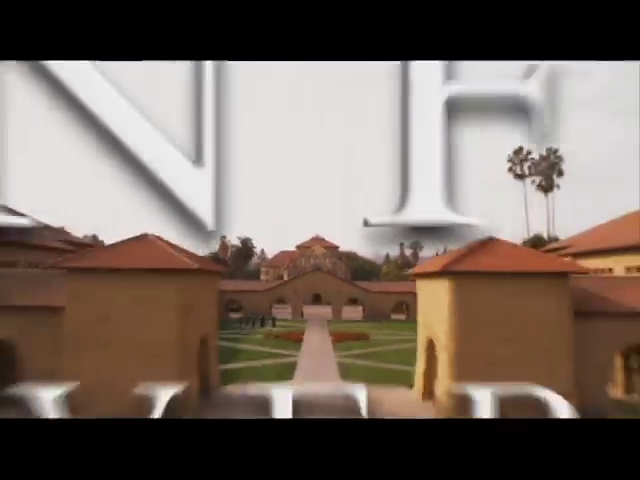
\includegraphics[width=0.78\textwidth]{lecture_02_figure_01.png}
  \caption{Reglas de diferencias finitas y sumas de Riemann que se usarán en el límite continuo posterior.}
  \lectureframe{00:04:20}
  \label{fig:l02-calculus-board}
\end{figure}

Estas son definiciones conocidas del cálculo. Aquí importa cómo escalan: \(\Delta x_i\) aporta un factor de \(\Delta\sigma\), mientras que una suma aporta un factor inverso al convertirse en integral.

\subsection{Extremos de Dirichlet y de Neumann}

El análisis de Fourier en un intervalo finito comienza por elegir las condiciones en los extremos. Dos opciones aparecerán repetidamente.

\begin{align}
  \text{Dirichlet:}\qquad
  &x(0)=x(\pi)=0,
  \label{eq:l02-dirichlet}\\
  \text{Neumann:}\qquad
  &\left.\partial_\sigma x\right|_{\sigma=0}
   =
   \left.\partial_\sigma x\right|_{\sigma=\pi}
   =0.
  \label{eq:l02-neumann}
\end{align}

Una cuerda de violín sujeta por ambos extremos ilustra el caso de Dirichlet: el desplazamiento se anula en los bordes. Una función de Neumann no tiene por qué anularse allí; su pendiente es cero en cada borde. En la pizarra se ven juntas las dos formas características.

\begin{figure}[H]
  \centering
  \begin{minipage}[t]{0.48\textwidth}
    \centering
    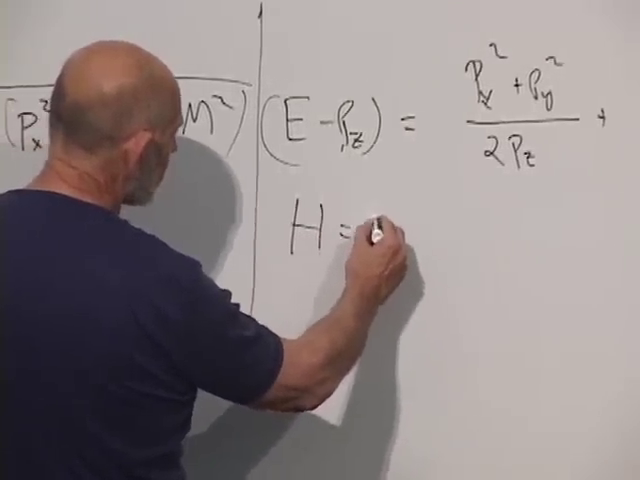
\includegraphics[width=\textwidth]{lecture_02_figure_02.png}
    \par\smallskip\footnotesize (a) Perfiles con extremos fijos y planos.
  \end{minipage}\hfill
  \begin{minipage}[t]{0.48\textwidth}
    \centering
    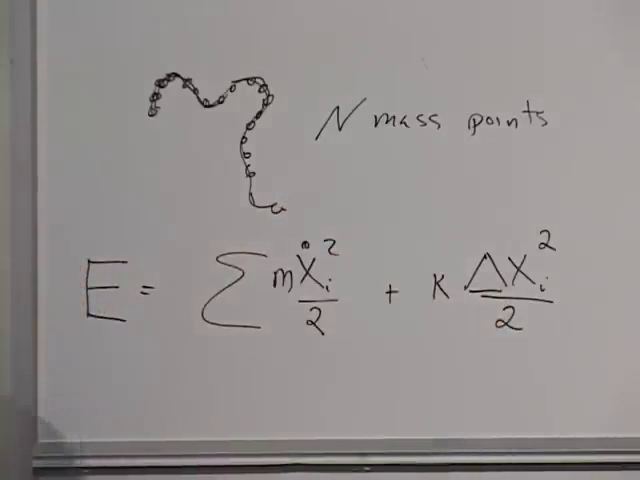
\includegraphics[width=\textwidth]{lecture_02_figure_03.png}
    \par\smallskip\footnotesize (b) Anillos ligeros que se deslizan sobre varillas verticales.
  \end{minipage}
  \caption{Condiciones de contorno representadas como formas y como sistemas mecánicos. El montaje de anillos deslizantes da un movimiento transversal inequívoco a un extremo libre.}
  \lectureframe{00:08:50 and 00:12:15}
  \label{fig:l02-boundaries-board}
\end{figure}

\begin{figure}[H]
  \centering
  \begin{adjustbox}{max width=\linewidth}
  \begin{tikzpicture}[>=Latex,thick,scale=0.92]
    \begin{scope}
      \draw[->] (0,0) -- (4.4,0) node[right] {\(\sigma\)};
      \draw[->] (0,-1.25) -- (0,1.35) node[above] {\(x\)};
      \draw[blue!70!black]
        (0,0) .. controls (0.8,1.1) and (1.4,1.0) .. (2.0,0)
        .. controls (2.7,-1.0) and (3.4,-0.8) .. (4.1,0);
      \fill (0,0) circle (0.06);
      \fill (4.1,0) circle (0.06);
      \node at (2.05,-1.65) {Dirichlet: \(x=0\)};
    \end{scope}
    \begin{scope}[xshift=5.8cm]
      \draw[->] (0,0) -- (4.4,0) node[right] {\(\sigma\)};
      \draw[->] (0,-1.25) -- (0,1.35) node[above] {\(x\)};
      \draw[orange!85!black]
        (0,0.65) .. controls (0.8,0.65) and (1.1,-0.9) .. (2.0,-0.9)
        .. controls (2.9,-0.9) and (3.2,0.55) .. (4.1,0.55);
      \draw[orange!85!black] (0,0.65) -- (0.45,0.65);
      \draw[orange!85!black] (3.65,0.55) -- (4.1,0.55);
      \node at (2.05,-1.65) {Neumann: \(\partial_\sigma x=0\)};
    \end{scope}
  \end{tikzpicture}
  \end{adjustbox}
  \caption{Para los datos de Dirichlet se fija el valor; para los de Neumann, la pendiente.}
  \label{fig:l02-boundaries-redraw}
\end{figure}

\begin{classroomqa}
\audiencequestion{¿Puede un tubo de órgano abierto o cerrado ofrecer un ejemplo claro de alguna de estas condiciones de contorno?\lecturetimestamp{00:09:19}}
\lecturerresponse{Puede, pero primero hay que especificar qué variable acústica se desarrolla. La perturbación de presión y el desplazamiento longitudinal obedecen condiciones idealizadas complementarias en un extremo abierto. En lugar de resolver esa cuestión secundaria en la pizarra, usemos el modelo de anillos deslizantes: anillos casi sin masa pueden moverse verticalmente sobre las varillas, de modo que los extremos de la cuerda quedan libres y el caso de Neumann resulta directo.}
\end{classroomqa}

\begin{classroomqa}
\audiencequestion{¿Puede la gráfica subir verticalmente y contener un salto brusco?\lecturetimestamp{00:09:53}}
\lecturerresponse{El análisis de Fourier admite saltos aislados en una función continua a trozos. Una cuerda física impone más restricciones. Un salto desconecta puntos vecinos y hace que la derivada espacial \(\partial_\sigma x\) sea singular en la energía continua que obtendremos más adelante. Por tanto, nos limitaremos a perfiles continuos y diferenciables.}
\end{classroomqa}

\begin{classroomqa}
\audiencequestion{¿Por qué el extremo abierto de un tubo, o cualquier extremo libre, debe satisfacer alguna condición de contorno?\lecturetimestamp{00:11:14}}
\lecturerresponse{El ejemplo acústico depende del campo elegido y dejamos sin resolver esa cuestión en la discusión. El ejemplo mecánico no presenta esa ambigüedad. Un anillo muy ligero puede deslizarse libremente, pero sigue unido al último tramo de cuerda. Deduciremos su condición a partir de la ley de Newton, en vez de darla por supuesta: una aceleración finita en el extremo obliga a que la pendiente se anule.}
\end{classroomqa}

\subsection{Las bases de Fourier}

Una vez fijada la clase de condiciones en los extremos, queda determinada la base de Fourier correspondiente. En \(0\leq\sigma\leq\pi\),

\begin{align}
  x_D(\sigma)
  &=
  \sum_{n=1}^{\infty}x_n\sin(n\sigma),
  \label{eq:l02-dirichlet-series}\\
  x_N(\sigma)
  &=
  \sum_{n=0}^{\infty}x_n\cos(n\sigma).
  \label{eq:l02-neumann-series}
\end{align}

Todos los senos de \eqref{eq:l02-dirichlet-series} se anulan en ambos extremos. Todas las funciones coseno de \eqref{eq:l02-neumann-series} tienen derivada nula en los extremos. Los límites inferiores son distintos por una razón: \(\sin(0\sigma)=0\) no aporta nada, mientras que \(\cos(0\sigma)=1\) es el modo constante, o de frecuencia nula. Este representa el valor medio de una función de Neumann.

\begin{figure}[H]
  \centering
  \begin{minipage}[t]{0.48\textwidth}
    \centering
    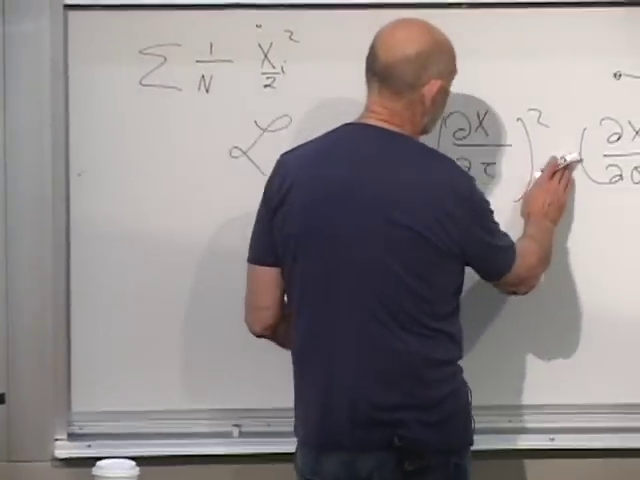
\includegraphics[width=\textwidth]{lecture_02_figure_04.png}
    \par\smallskip\footnotesize (a) Desarrollos en senos y cosenos.
  \end{minipage}\hfill
  \begin{minipage}[t]{0.48\textwidth}
    \centering
    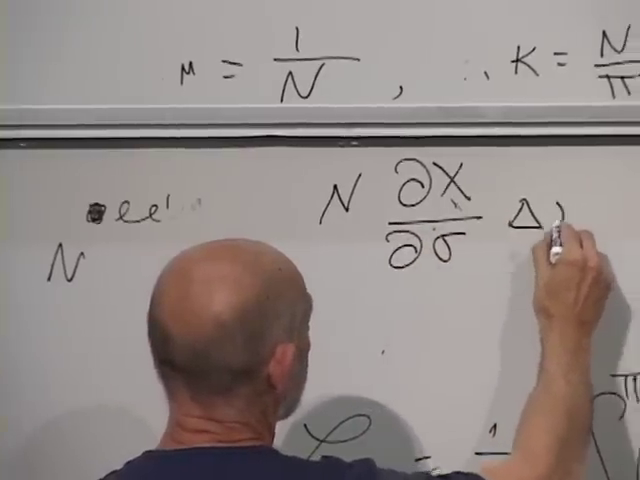
\includegraphics[width=\textwidth]{lecture_02_figure_05.png}
    \par\smallskip\footnotesize (b) Ortogonalidad y el modo constante excepcional.
  \end{minipage}
  \caption{Propiedades de Fourier que usaremos después para diagonalizar la cuerda.}
  \lectureframe{00:16:15 and 00:20:30}
  \label{fig:l02-fourier-board}
\end{figure}

La derivación intercambia las dos clases:

\begin{equation}
  \begin{aligned}
    \partial_\sigma\sin(n\sigma)&=n\cos(n\sigma),\\
    \partial_\sigma\cos(n\sigma)&=-n\sin(n\sigma).
  \end{aligned}
  \label{eq:l02-basis-derivatives}
\end{equation}

Así, la derivada de una serie de Dirichlet tiene comportamiento de Neumann, y la derivada de una serie de Neumann tiene comportamiento de Dirichlet. La ortogonalidad elimina entonces los términos cruzados entre modos distintos:

\begin{align}
  \int_0^\pi\cos(n\sigma)\cos(m\sigma)\,d\sigma
  &=
  \frac{\pi}{2}\delta_{nm},
  && n,m\geq1,
  \label{eq:l02-cos-orthogonality}\\
  \int_0^\pi\sin(n\sigma)\sin(m\sigma)\,d\sigma
  &=
  \frac{\pi}{2}\delta_{nm},
  && n,m\geq1,
  \label{eq:l02-sin-orthogonality}\\
  \int_0^\pi 1\,d\sigma&=\pi .
  \label{eq:l02-zero-norm}
\end{align}

La última línea corresponde a la norma excepcional del coseno \(n=m=0\). Una constante no se normaliza igual que un armónico no nulo, y ese factor de dos distinguirá el modo del centro de masas de la cuerda de sus modos internos.

\subsection{Una fórmula de oscilador para recordar}

Tras reescalar una coordenada para que la masa mecánica sea uno, un oscilador que obedece la ley de Hooke tiene

\begin{align}
  E_{\mathrm{osc}}
  &=
  \frac12\dot q^{\,2}
  +\frac12\omega^2q^2,
  \label{eq:l02-oscillator-energy}\\
  L_{\mathrm{osc}}
  &=
  \frac12\dot q^{\,2}
  -\frac12\omega^2q^2.
  \label{eq:l02-oscillator-lagrangian}
\end{align}

\begin{figure}[H]
  \centering
  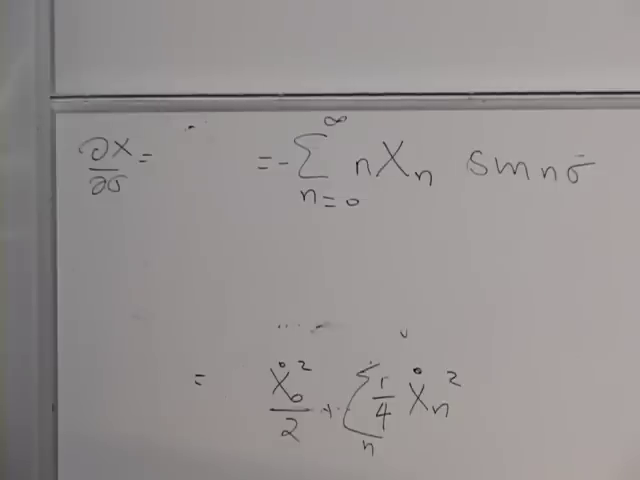
\includegraphics[width=0.68\textwidth]{lecture_02_figure_06.png}
  \caption{La energía del oscilador, escrita de modo que el coeficiente de \(q^2\) permite identificar directamente \(\omega^2\).}
  \lectureframe{00:24:00}
  \label{fig:l02-oscillator-board}
\end{figure}

Clásicamente, \(\omega=\sqrt{\kappa/m}\); el reescalamiento de la coordenada ha fijado \(m=1\). En mecánica cuántica,

\begin{equation}
  E_Q=\hbar\omega\left(Q+\frac12\right),
  \qquad Q=0,1,2,\ldots .
  \label{eq:l02-oscillator-spectrum}
\end{equation}

Para las separaciones entre niveles podemos restar el término común del estado fundamental y decir que cada cuanto cuesta \(\hbar\omega\). El cálculo de la cuerda hará exactamente eso al principio y dejará para más adelante la energía total de punto cero.

\begin{classroomqa}
\audiencequestion{¿Cómo se obtiene la frecuencia del oscilador a partir de la fórmula de la energía?\lecturetimestamp{00:23:21}}
\lecturerresponse{Antes del reescalamiento es \(\omega=\sqrt{\kappa/m}\). Con masa unidad, el término del potencial es \(\frac12\omega^2q^2\), por lo que su coeficiente cuadrático es el cuadrado de la frecuencia.}
\end{classroomqa}

\section{¿Qué hace que un sistema compuesto sea una partícula?}

Una cuerda es extensa y la modelaremos con muchas partes acopladas. ¿En qué sentido puede ser partícula uno de sus estados cuánticos? La puntualidad no puede ser el criterio decisivo. Los protones y los neutrones son compuestos. Los electrones y los fotones están acompañados por el vestido de los campos cuánticos, aunque no se haya resuelto ninguna subestructura intrínseca. La imagen clásica de un punto geométrico rodeado de vacío no es la adecuada para una excitación cuántica.

Tampoco bastan la masa y la posición del centro de masas. Una caja cerrada de gas tiene ambas. Una taza de café también. Normalmente no llamamos partícula a ninguna de las dos. La indivisibilidad tampoco sirve, porque un protón es divisible, y el espín no distingue las partículas microscópicas de los cuerpos macroscópicos.

El criterio útil es el aislamiento espectral. Representemos la energía en reposo en un eje vertical y preguntemos cuánta energía hace falta para llegar a otro estado interno. No hay una sucesión de excitaciones del electrón, accesibles experimentalmente y situadas justo por encima de él. El protón sí tiene resonancias, pero las primeras cuestan unos cientos de MeV, una fracción considerable de la masa del protón. Los estados están lo bastante separados como para identificarlos individualmente.

Una taza de café es lo contrario. Se puede añadir una cantidad arbitrariamente pequeña de energía a un modo sonoro de gran longitud de onda, desplazar una molécula o producir un fonón. Hay cantidades enormes de estados concentrados en un intervalo diminuto. A escala de laboratorio forman un continuo. Esta es la distinción práctica entre una partícula y una \emph{masa informe}.

\begin{figure}[H]
  \centering
  \includegraphics[width=0.58\textwidth]{lecture_02_figure_07.png}
  \caption{Eje vertical de energía en la pizarra al comparar un nivel aislado de una partícula con las numerosas excitaciones de la materia ordinaria.}
  \lectureframe{00:31:10}
  \label{fig:l02-spectrum-board}
\end{figure}

\begin{figure}[H]
  \centering
  \begin{adjustbox}{max width=\linewidth}
  \begin{tikzpicture}[>=Latex,thick]
    \begin{scope}
      \draw[->] (0,0) -- (0,4.8) node[above] {energy};
      \draw[blue!70!black,line width=1.2pt] (-1.0,0.65) -- (1.0,0.65);
      \draw[blue!70!black,line width=1.2pt] (-1.0,3.65) -- (1.0,3.65);
      \node[right] at (1.05,0.65) {ground state};
      \node[right] at (1.05,3.65) {first internal excitation};
      \draw[<->] (0.65,0.75) -- (0.65,3.55)
        node[midway,right] {large gap};
      \node at (0,-0.55) {particle-like};
    \end{scope}
    \begin{scope}[xshift=7.0cm]
      \draw[->] (0,0) -- (0,4.8) node[above] {energy};
      \foreach \y in {0.55,0.69,0.82,0.94,1.05,1.15,1.24,1.32,1.39,1.45,
        1.51,1.57,1.63,1.70,1.78,1.87,1.97,2.09,2.22,2.36,2.51,2.67,2.84,
        3.02,3.21,3.41,3.62,3.84,4.07}
        \draw[orange!85!black] (-0.95,\y) -- (0.95,\y);
      \node[right] at (1.05,2.25) {dense phonon and internal states};
      \node at (0,-0.55) {macroscopic matter};
    \end{scope}
  \end{tikzpicture}
  \end{adjustbox}
  \caption{El criterio operativo de partícula empleado en la lección es el aislamiento espectral, no la puntualidad literal.}
  \label{fig:l02-particle-redraw}
\end{figure}

Este criterio convierte la cuestión filosófica en un cálculo. Cuantizamos la cuerda, hallamos sus niveles de energía interna y examinamos su separación. Si el primer estado excitado de la cuerda está cerca de la escala de Planck mientras que el estado fundamental observado es ligero, la brecha supera en más de veinte órdenes de magnitud las energías actuales de los aceleradores. En el régimen accesible, la cuerda se comporta entonces como una partícula elemental.

\begin{classroomqa}
\audiencequestion{¿El comportamiento de partícula depende únicamente de la escala de observación? Si ampliamos lo suficiente, ¿dejan los niveles de estar separados?\lecturetimestamp{00:33:33}}
\lecturerresponse{Ampliar la imagen puede revelar que un objeto tiene muchos constituyentes, pero no elimina el espectro. La comparación pertinente es entre la resolución energética del experimento y la brecha hasta la primera excitación interna. Un objeto compuesto puede seguir comportándose como una partícula si esa brecha es enorme.}
\end{classroomqa}

\begin{classroomqa}
\audiencequestion{¿Por qué una cuerda de violín ordinaria no es una partícula?\lecturetimestamp{00:34:37}}
\lecturerresponse{La energía de un cuanto vibracional es inconmensurablemente pequeña comparada con la energía en reposo de la cuerda macroscópica. Por tanto, caben muchos estados cuánticos en un intervalo relativo diminuto. La cuerda pertenece al lado denso de la comparación espectral, no al lado aislado.}
\end{classroomqa}

\begin{classroomqa}
\audiencequestion{¿Son partículas puntuales los fotones y los electrones si los campos cuánticos los rodean con fluctuaciones virtuales?\lecturetimestamp{00:35:40}}
\lecturerresponse{La palabra clásica \emph{punto} está cargando con demasiado significado. El electrón y el fotón físicos son excitaciones de campo vestidas; sin embargo, los experimentos no han encontrado en ninguno una estructura intrínseca de constituyentes ni un factor de forma finito. Para el argumento que nos ocupa, lo relevante es que ninguno tiene una densa torre de estados internos casi degenerados.\editorialnote{La conferencia relaciona el momento magnético anómalo del electrón con una borrosidad cuántica medible. En la terminología moderna, el momento anómalo es un efecto de vestidura radiativa, no una prueba de que se haya resuelto un radio finito del electrón. Convencionalmente, «puntual» significa que no se ha detectado subestructura intrínseca ni factor de forma hasta la escala estudiada.}}
\end{classroomqa}

\begin{classroomqa}
\audiencequestion{¿Depende el tamaño de un fotón de su frecuencia?\lecturetimestamp{00:36:49}}
\lecturerresponse{Desde luego, su longitud de onda sí depende de ella. Eso es distinto del tamaño intrínseco de sus constituyentes. Cambiar la frecuencia modifica el paquete de ondas y su longitud de onda, no un radio interno del fotón que se haya podido resolver.}
\end{classroomqa}

\section{Mecánica transversal exacta a gran momento}

Volvamos ahora a la dificultad relativista. No se puede tratar un bastón que gira rápidamente de forma no relativista solo por situar su centro de masas en reposo. Sus extremos siguen moviéndose uno respecto del otro a velocidades relativistas. La aproximación no relativista falla debido al movimiento relativo interno.

Sin embargo, existe otro límite. Elijamos un eje \(z\) y apliquemos un impulso de Lorentz al sistema completo, llevándolo a un momento longitudinal positivo muy grande \(P_z\). Mantengamos finito su momento transversal

\begin{equation}
  p_\perp^2=p_x^2+p_y^2
\end{equation}

 . En el límite \(P_z\to\infty\), la proyección transversal admite entonces una formulación hamiltoniana exactamente no relativista, aunque el movimiento interno sin impulso fuera relativista.

\begin{classroomqa}
\audiencequestion{¿Significa el momento infinito que el sistema masivo alcanza realmente la velocidad de la luz?\lecturetimestamp{00:40:43}}
\lecturerresponse{Ningún impulso finito lo consigue. Se construyen magnitudes con límites bien definidos cuando \(P_z\) crece sin límite. La expresión designa un procedimiento límite, no un estado físico finito con \(v=c\).}
\end{classroomqa}

\begin{classroomqa}
\audiencequestion{¿Qué eje hay que elegir, y qué ocurre si el objeto gira alrededor de ese eje o en torno a otro que lo cruza?\lecturetimestamp{00:41:14}}
\lecturerresponse{Se puede elegir cualquier eje e impulsar el sistema completo a lo largo de él. La mecánica que queda explícita es la de la proyección sobre el plano perpendicular. Una varilla que gira puede parecer acortada o barrer ese plano, pero su proyección transversal tiene forma no relativista.}
\end{classroomqa}

Las cuerdas tienen una propiedad adicional que hace que esta representación sea especialmente potente. En el calibre de frente de luz, las coordenadas longitudinales internas no son osciladores independientes. Las ligaduras las determinan a partir del movimiento transversal. Por tanto, basta conocer la cuerda transversal para reconstruir los grados de libertad físicos.

\begin{classroomqa}
\audiencequestion{¿La ausencia de una coordenada longitudinal independiente significa que la cuerda está simplemente atrapada en un sándwich delgado?\lecturetimestamp{00:42:26}}
\lecturerresponse{La contracción de Lorentz sí hace pequeño su tamaño longitudinal en el sistema de referencia impulsado, pero la afirmación va más allá. Todo movimiento longitudinal residual está condicionado por el movimiento transversal; no se puede especificar de manera independiente.}
\end{classroomqa}

\begin{classroomqa}
\audiencequestion{¿Está relacionada esta reducción a datos transversales con el principio holográfico?\lecturetimestamp{00:43:12}}
\lecturerresponse{Está estrechamente relacionada con la línea de pensamiento que condujo a las ideas holográficas, aunque desarrollar esa conexión nos apartaría del cálculo actual. Aquí solo sirve para justificar que trabajemos con la cuerda transversal.}
\end{classroomqa}

\subsection{Restar el impulso y reescalar el tiempo}

Sea \(M\) la masa invariante del sistema completo, que incluye las masas de los constituyentes, la energía cinética y la energía de enlace. En unidades \(c=1\),

\begin{equation}
  E=\sqrt{P_z^2+p_\perp^2+M^2}.
  \label{eq:l02-relativistic-energy}
\end{equation}

Para valores de \(P_z\) mucho mayores que los de \(p_\perp\) y \(M\),

\begin{equation}
  E
  =
  P_z+\frac{p_\perp^2+M^2}{2P_z}
  +O(P_z^{-3}).
  \label{eq:l02-large-pz}
\end{equation}

\begin{figure}[H]
  \centering
  \includegraphics[width=0.76\textwidth]{lecture_02_figure_08.png}
  \caption{La expansión completa en gran \(P_z\), conservando el momento transversal y la masa invariante.}
  \lectureframe{00:47:30}
  \label{fig:l02-large-pz-board}
\end{figure}

El término dominante es grande, pero no contiene información sobre el estado interno. En un proceso que conserva \(P_z\), como una transición entre niveles internos de un átomo impulsado sin cambiar su momento longitudinal total, ese término se cancela en todas las diferencias de energía. Por tanto, estudiamos

\begin{equation}
  E-P_z=\frac{p_\perp^2+M^2}{2P_z}+O(P_z^{-3}).
  \label{eq:l02-residual-energy}
\end{equation}

El denominador tiene significado físico. Como el hamiltoniano genera la evolución temporal, la pequeña energía residual indica que la evolución interna parece lenta en el tiempo de laboratorio. Esto es la dilatación temporal. Para conservar el movimiento interno, introduzcamos un parámetro de evolución reescalado \(\tau\) o, de forma equivalente, multipliquemos el hamiltoniano residual por \(P_z\):

\begin{equation}
  H_\perp
  \equiv
  \lim_{P_z\to\infty}P_z(E-P_z)
  =
  \frac12p_\perp^2+\frac12M^2.
  \label{eq:l02-transverse-hamiltonian}
\end{equation}

\begin{figure}[H]
  \centering
  \begin{minipage}[t]{0.48\textwidth}
    \centering
    \includegraphics[width=\textwidth]{lecture_02_figure_09.png}
    \par\smallskip\footnotesize (a) \(H=i\partial_t\) y la evolución interna ralentizada.
  \end{minipage}\hfill
  \begin{minipage}[t]{0.48\textwidth}
    \centering
    \includegraphics[width=\textwidth]{lecture_02_figure_10.png}
    \par\smallskip\footnotesize (b) El hamiltoniano transversal finito tras reescalar el tiempo.
  \end{minipage}
  \caption{De la energía residual dilatada en el tiempo a un hamiltoniano finito en dos dimensiones.}
  \lectureframe{00:49:20 and 00:52:40}
  \label{fig:l02-lightfront-board}
\end{figure}

Esta es exactamente la forma de la energía de una partícula de masa unidad que se mueve en dos dimensiones: energía cinética \(p_\perp^2/2\) más energía interna \(M^2/2\). Lo inusual es el cuadrado. En esta descripción, la magnitud que desempeña el papel de la energía en reposo o de enlace es proporcional al cuadrado de la masa invariante.\editorialnote{Con las variables convencionales de frente de luz \(P^\pm=(E\pm P_z)/\sqrt2\), la relación exacta de la capa de masa es \(2P^+P^-=p_\perp^2+M^2\). La ecuación \eqref{eq:l02-transverse-hamiltonian} es la normalización para \(P_z\) grande de la misma relación invariante que se emplea en la lección.}

\begin{classroomqa}
\audiencequestion{¿Qué ocurre con los momentos longitudinales de las partes individuales de un sistema compuesto?\lecturetimestamp{00:51:30}}
\lecturerresponse{Para un objeto compuesto genérico hay que conservar las fracciones del momento longitudinal total \(P_z\) que llevan sus constituyentes. La fórmula anterior utiliza el momento total del centro de masas. La teoría de cuerdas es especial porque sus ligaduras determinan el movimiento longitudinal relativo a partir de los grados de libertad transversales, de modo que no hay que añadir ningún oscilador longitudinal independiente.}
\end{classroomqa}

\section{Una cuerda abierta discreta}

La cuerda impulsada ahora solo se mueve explícitamente en el plano transversal. Denominemos sus dos coordenadas \(X\) y \(Y\), y aproximémosla primero mediante \(N\) puntos materiales unidos por \(N-1\) resortes. Si \(\mu\) es la masa análoga de cada punto y \(k\) la constante del resorte entre vecinos, la energía es

\begin{equation}
  E_N
  =
  \sum_i
  \left[
    \frac{\mu}{2}
    \left(\dot X_i^2+\dot Y_i^2\right)
    +
    \frac{k}{2}
    \left((\Delta X_i)^2+(\Delta Y_i)^2\right)
  \right].
  \label{eq:l02-discrete-energy}
\end{equation}

Cada término en \(X\) tiene un término idéntico en \(Y\), porque el plano transversal tiene dos direcciones. El índice \(i\) identifica un punto de la cadena; no es una coordenada espacial.

\begin{figure}[H]
  \centering
  \begin{minipage}[t]{0.48\textwidth}
    \centering
    \includegraphics[width=\textwidth]{lecture_02_figure_11.png}
    \par\smallskip\footnotesize (a) La cadena de cuentas y su energía discreta.
  \end{minipage}\hfill
  \begin{minipage}[t]{0.48\textwidth}
    \centering
    \includegraphics[width=\textwidth]{lecture_02_figure_12.png}
    \par\smallskip\footnotesize (b) El escalamiento para valores grandes de \(N\) de \(\mu\) y
    \(k\).
  \end{minipage}
  \caption{La cuerda abierta regularizada antes de tomar el límite continuo.}
  \lectureframe{00:57:42 and 01:02:40}
  \label{fig:l02-chain-board}
\end{figure}

\begin{figure}[H]
  \centering
  \begin{adjustbox}{max width=\linewidth}
  \begin{tikzpicture}[>=Latex,thick]
    \foreach \i in {0,...,8} {
      \coordinate (p\i) at ({1.05*\i},{0.30*sin(55*\i)});
      \filldraw[white] (p\i) circle (0.10);
      \draw (p\i) circle (0.10);
    }
    \foreach \i in {0,...,7} {
      \pgfmathtruncatemacro{\j}{\i+1}
      \draw[decorate,decoration={zigzag,segment length=4pt,amplitude=2pt}]
        (p\i) -- (p\j);
    }
    \node[above=0.35cm of p0] {\(i=0\)};
    \node[above=0.35cm of p8] {\(i=N-1\)};
    \draw[<->] (0,-1.15) -- (8.4,-1.15)
      node[midway,below] {\(0\leq\sigma\leq\pi\)};
    \node at (4.2,1.25)
      {\(\mu=1/N,\quad k=N/\pi^2,\quad\Delta\sigma=\pi/N\)};
  \end{tikzpicture}
  \end{adjustbox}
  \caption{Una imagen clara de la regularización. Al refinar la cadena, los puntos se hacen más ligeros y los resortes microscópicos más rígidos.}
  \label{fig:l02-chain-redraw}
\end{figure}

El parámetro \(\sigma\) indica la posición a lo largo de la cadena. Elegir \(0\leq\sigma\leq\pi\) es una convención, no una medición de longitud física. Nos recuerda que la cuerda tiene dos extremos. Más adelante, la cuerda cerrada se parametrizará periódicamente en \(0\leq\sigma<2\pi\).

El límite continuo debe conservar finita la mecánica colectiva. Si la masa de cada cuenta fuera fija, la masa análoga total divergiría; por tanto, elijamos

\begin{equation}
  \mu=\frac{1}{N}.
  \label{eq:l02-mu-scaling}
\end{equation}

Entonces \(N\mu=1\). No es la masa en reposo relativista \(M\); es el coeficiente de inercia del modelo transversal análogo.

Al aumentar su número, los resortes en serie se vuelven más blandos. Para mantener finita la rigidez de la cadena completa, cada resorte microscópico debe hacerse más rígido:

\begin{equation}
  k=\frac{N}{\pi^2}
  =\frac{1}{\pi\,\Delta\sigma}.
  \label{eq:l02-k-scaling}
\end{equation}

Solo es esencial \(k\propto N\). El factor \(\pi^2\) es una normalización elegida para eliminar factores \(\pi\) sobrantes de las fórmulas del continuo.

\begin{classroomqa}
\audiencequestion{¿Es \(\mu\) la masa en reposo física de cada punto de la cuerda?\lecturetimestamp{01:10:34}}
\lecturerresponse{No. Es la masa análoga no relativista que aparece en la cadena transversal. Llamarla \(M\) llevaría a confundirla con la masa invariante en reposo del estado completo de la cuerda relativista. Su única función aquí es producir la inercia continua correcta.}
\end{classroomqa}

\section{El sistema de ondas continuo}

Apliquemos las reglas preparadas al comienzo. Como \(1/N=\Delta\sigma/\pi\),

\begin{align}
  \sum_i\frac{\mu}{2}\dot X_i^2
  &=
  \frac{1}{2\pi}
  \sum_i\dot X_i^2\,\Delta\sigma
  \longrightarrow
  \frac{1}{2\pi}
  \int_0^\pi
  \left(\partial_\tau X\right)^2d\sigma ,
  \label{eq:l02-kinetic-limit}\\
  \sum_i\frac{k}{2}(\Delta X_i)^2
  &\longrightarrow
  \frac{1}{2\pi}
  \int_0^\pi
  \left(\partial_\sigma X\right)^2d\sigma .
  \label{eq:l02-potential-limit}
\end{align}

Para la segunda línea, usemos \(\Delta X_i=\partial_\sigma X\,\Delta\sigma\) junto con \(k=1/(\pi\Delta\sigma)\). El mismo cálculo se aplica a \(Y\).

\begin{figure}[H]
  \centering
  \begin{minipage}[t]{0.48\textwidth}
    \centering
    \includegraphics[width=\textwidth]{lecture_02_figure_13.png}
    \par\smallskip\footnotesize (a) Reemplazos de sumas por integrales y de diferencias por derivadas.
  \end{minipage}\hfill
  \begin{minipage}[t]{0.48\textwidth}
    \centering
    \includegraphics[width=\textwidth]{lecture_02_figure_14.png}
    \par\smallskip\footnotesize (b) La energía continua completa.
  \end{minipage}
  \caption{La cadena discreta se convierte en un campo definido en el intervalo \(\sigma\).}
  \lectureframe{01:05:40 and 01:07:00}
  \label{fig:l02-continuum-board}
\end{figure}

La energía y el lagrangiano resultantes son

\begin{align}
  E
  &=
  \frac{1}{2\pi}
  \int_0^\pi d\sigma\,
  \left[
    (\partial_\tau X)^2+(\partial_\tau Y)^2\right.\notag\\[-0.25em]
  &\hspace{6.5em}\left.
    +(\partial_\sigma X)^2+(\partial_\sigma Y)^2
  \right],
  \label{eq:l02-continuum-energy}\\
  L
  &=
  \frac{1}{2\pi}
  \int_0^\pi d\sigma\,
  \left[
    (\partial_\tau X)^2+(\partial_\tau Y)^2\right.\notag\\[-0.25em]
  &\hspace{6.5em}\left.
    -(\partial_\sigma X)^2-(\partial_\sigma Y)^2
  \right].
  \label{eq:l02-continuum-lagrangian}
\end{align}

\begin{figure}[H]
  \centering
  \includegraphics[width=0.78\textwidth]{lecture_02_figure_15.png}
  \caption{El lagrangiano continuo, con los términos cinético y de estiramiento de signos opuestos.}
  \lectureframe{01:08:48}
  \label{fig:l02-lagrangian-board}
\end{figure}

Si cambiamos el nombre de \(\sigma\) por el de una coordenada espacial ordinaria y llamamos \(X\) al campo \(\phi\), estas son la energía y el lagrangiano de un campo de ondas unidimensional. Al variar \eqref{eq:l02-continuum-lagrangian} se obtiene

\begin{equation}
  \left(\partial_\tau^2-\partial_\sigma^2\right)X=0,
  \qquad
  \left(\partial_\tau^2-\partial_\sigma^2\right)Y=0.
  \label{eq:l02-wave-equation}
\end{equation}

No hace falta resolver directamente estas ecuaciones para el argumento inmediato. Basta con la imagen útil de ondas que viajan a izquierda y derecha a lo largo de la cuerda y se reflejan en los extremos. Una reflexión de Dirichlet invierte el signo del desplazamiento; una de Neumann lo conserva.

\begin{classroomqa}
\audiencequestion{¿Qué significa exactamente la variable temporal \(\tau\)?\lecturetimestamp{01:08:54}}
\lecturerresponse{Es el tiempo reescalado que se usa para seguir el movimiento interno en la descripción de momento longitudinal \(P_z\) grande. Un reloj impulsado junto con el sistema marcha lentamente respecto del tiempo de laboratorio; \(\tau\) elimina esa dilatación para que las oscilaciones internas conserven una frecuencia finita. Para esta mecánica transversal se puede tratar simplemente como el tiempo.\editorialnote{En la lección se llama informalmente tiempo propio a \(\tau\). Para una cuerda extensa, el parámetro preciso de evolución en el frente de luz es un tiempo reescalado y fijado por el calibre, no un único tiempo propio invariante compartido por todos los puntos. El argumento pretendido sobre la dilatación temporal no cambia.}}\end{classroomqa}

Cuando el centro de masas está en reposo en el plano transversal, la parte interna de \eqref{eq:l02-continuum-energy} es proporcional a \(M^2\), con la normalización de \eqref{eq:l02-transverse-hamiltonian}. Por eso, al cuantizar este sistema de ondas aparentemente ordinario aparecerá el espectro relativista de masas.

\begin{classroomqa}
\audiencequestion{¿Tiene nombre \(P_z(E-P_z)\)?\lecturetimestamp{01:11:00}}
\lecturerresponse{Se suele llamar energía de cono de luz o energía de frente de luz. «Frente de luz» describe mejor el plano nulo que se usa como superficie de evolución; la terminología tradicional no es importante para el cálculo.}
\end{classroomqa}

\begin{classroomqa}
\audiencequestion{¿La palabra «cono» se refiere al cono de luz habitual del espacio-tiempo, y fue Dirac quien introdujo esta terminología?\lecturetimestamp{01:11:17}}
\lecturerresponse{La construcción con coordenadas nulas puede dibujarse con ejes a 45 grados, pero la superficie de evolución aquí es un frente de luz, no el cono completo en expansión. Dirac desarrolló formulaciones relacionadas de la dinámica relativista; la cuestión histórica sobre el nombre quedó abierta y no afecta a las ecuaciones.}
\end{classroomqa}

\section{Por qué un extremo libre satisface la condición de Neumann}

Ahora podemos deducir la condición en los extremos en vez de postularla. La ley de Newton es aplicable porque la mecánica transversal impulsada tiene exactamente forma no relativista. Un punto material interior recibe el tirón de resortes a ambos lados. El punto del extremo solo recibe el tirón del resorte que lo une a su vecino.

\begin{classroomqa}
\audiencequestion{¿Por qué podemos usar la ley de Newton al hablar de una cuerda relativista?\lecturetimestamp{01:14:52}}
\lecturerresponse{No estamos aplicando la mecánica newtoniana al movimiento completo en el espacio-tiempo sin impulso. La aplicamos a las variables transversales de la descripción de momento infinito, cuyo hamiltoniano tiene exactamente forma no relativista.}
\end{classroomqa}

En el extremo derecho, la ley de Hooke da, salvo por la orientación,

\begin{equation}
  F_{\mathrm{end}}
  =
  -k\,\Delta X
  =
  -\frac{1}{\pi\Delta\sigma}
   \left(\partial_\sigma X\,\Delta\sigma\right)
  =
  -\frac{1}{\pi}\partial_\sigma X .
  \label{eq:l02-endpoint-force}
\end{equation}

\begin{figure}[H]
  \centering
  \begin{minipage}[t]{0.48\textwidth}
    \centering
    \includegraphics[width=\textwidth]{lecture_02_figure_16.png}
    \par\smallskip\footnotesize Fuerza en el extremo proporcional a la pendiente local.
  \end{minipage}\hfill
  \begin{minipage}[t]{0.48\textwidth}
    \centering
    \includegraphics[width=\textwidth]{lecture_02_figure_17.png}
    \par\smallskip\footnotesize La condición de aceleración finita.
  \end{minipage}
  \caption{Deducción de la condición de contorno en el extremo libre a partir de la ley de Newton.}
  \lectureframe{01:18:20 and 01:20:10}
  \label{fig:l02-neumann-board}
\end{figure}

La ecuación de Newton para el punto del extremo es

\begin{equation}
  \mu\,\partial_\tau^2X=F_{\mathrm{end}},
  \qquad
  \mu=\frac1N=\frac{\Delta\sigma}{\pi}.
  \label{eq:l02-endpoint-newton}
\end{equation}

Combinando \eqref{eq:l02-endpoint-force} y \eqref{eq:l02-endpoint-newton},

\begin{equation}
  \partial_\sigma X
  =
  -\Delta\sigma\,\partial_\tau^2X
  \quad\text{at the right endpoint},
  \label{eq:l02-endpoint-scaling}
\end{equation}

con el signo de la fuerza invertido en el extremo izquierdo. Si \(\partial_\sigma X\) tendiera a una constante distinta de cero cuando \(\Delta\sigma\to0\), la aceleración del extremo divergiría como \(N\). Por tanto, un límite continuo razonable con aceleración finita exige

\begin{equation}
  \left.\partial_\sigma X\right|_{0,\pi}=0,
  \qquad
  \left.\partial_\sigma Y\right|_{0,\pi}=0.
  \label{eq:l02-open-neumann}
\end{equation}

\begin{figure}[H]
  \centering
  \begin{adjustbox}{max width=\linewidth}
  \begin{tikzpicture}[>=Latex,thick,scale=1.0]
    \coordinate (a) at (0,0);
    \coordinate (b) at (4.5,0.75);
    \filldraw[white] (a) circle (0.12);
    \draw (a) circle (0.12);
    \filldraw[white] (b) circle (0.12);
    \draw (b) circle (0.12);
    \draw[decorate,decoration={zigzag,segment length=6pt,amplitude=3pt}]
      (a) -- (b);
    \draw[dashed] (a) -- (0,-1.2);
    \draw[dashed] (b) -- (4.5,-1.2);
    \draw[<->] (4.85,0) -- (4.85,0.75)
      node[midway,right] {\(\Delta X\)};
    \draw[->,red!70!black] (b) -- (5.75,0.95)
      node[right] {\(F_{\rm end}=-k\Delta X\)};
    \node[below] at (0,-1.2) {\(N-1\)};
    \node[below] at (4.5,-1.2) {\(N\)};
    \node at (2.5,-2.0)
      {\(\mu\ddot X=-k\Delta X
      \ \Longrightarrow\
      \partial_\sigma X=-\Delta\sigma\,\ddot X\to0\)};
  \end{tikzpicture}
  \end{adjustbox}
  \caption{En el límite del regulador, la masa del último punto se anula. Solo es posible una aceleración finita si la pendiente en el extremo se anula.}
  \label{fig:l02-neumann-redraw}
\end{figure}

El mismo argumento en ambos extremos y en las dos direcciones transversales da lugar a condiciones de contorno de Neumann para una cuerda abierta libre.

\section{Modos normales de la cuerda abierta}

Ya tenemos un sistema clásico completo: un lagrangiano y sus condiciones de contorno. La cuantización se simplifica tras aplicar el análisis de Fourier. Como los extremos son de Neumann,

\begin{align}
  X(\sigma,\tau)
  &=
  \sum_{n=0}^{\infty}X_n(\tau)\cos(n\sigma),
  \label{eq:l02-X-expansion}\\
  Y(\sigma,\tau)
  &=
  \sum_{n=0}^{\infty}Y_n(\tau)\cos(n\sigma).
  \label{eq:l02-Y-expansion}
\end{align}

Los cosenos contienen toda la dependencia de \(\sigma\). Los coeficientes contienen toda la dependencia temporal; la cuerda oscila porque cambian \(X_n(\tau)\) y \(Y_n(\tau)\).

\begin{figure}[H]
  \centering
  \includegraphics[width=0.78\textwidth]{lecture_02_figure_18.png}
  \caption{La expansión en modos de Neumann, junto a la regla de ortogonalidad que reducirá las sumas dobles.}
  \lectureframe{01:21:45}
  \label{fig:l02-mode-expansion-board}
\end{figure}

\subsection{Término cinético y modo cero}

Al derivar respecto del tiempo, se obtiene

\begin{equation}
  \partial_\tau X
  =
  \sum_{n=0}^{\infty}\dot X_n(\tau)\cos(n\sigma).
  \label{eq:l02-time-mode}
\end{equation}

Al elevar al cuadrado aparece una suma doble sobre \(n\) y \(m\), pero
\eqref{eq:l02-cos-orthogonality} elimina todos los términos con \(n\neq m\).
Separando el modo constante,

\begin{equation}
  \frac{1}{2\pi}\int_0^\pi
  (\partial_\tau X)^2\,d\sigma
  =
  \frac12\dot X_0^{\,2}
  +
  \frac14\sum_{n=1}^{\infty}\dot X_n^{\,2}.
  \label{eq:l02-mode-kinetic}
\end{equation}

\begin{figure}[H]
  \centering
  \includegraphics[width=0.76\textwidth]{lecture_02_figure_19.png}
  \caption{La integral de ortogonalidad reduce la suma doble cinética al modo cero más una suma diagonal.}
  \lectureframe{01:29:10}
  \label{fig:l02-mode-kinetic-board}
\end{figure}

El coeficiente constante es la posición media,

\begin{equation}
  X_0(\tau)=\frac1\pi\int_0^\pi X(\sigma,\tau)\,d\sigma ,
  \label{eq:l02-center-of-mass}
\end{equation}

y, de manera análoga, para \(Y_0\). Con una densidad de masa uniforme análoga, estas son las coordenadas del centro de masas. Tienen energía cinética, pero no fuerza restauradora: toda la cuerda puede moverse libremente por el plano transversal.

\subsection{Término de tensión y frecuencias de los osciladores}

Al derivar respecto de la posición, se obtiene

\begin{equation}
  \partial_\sigma X
  =
  -\sum_{n=1}^{\infty}nX_n(\tau)\sin(n\sigma).
  \label{eq:l02-spatial-mode}
\end{equation}

El modo cero desaparece porque una traslación uniforme no estira la cuerda. Usando la ortogonalidad de los senos,

\begin{equation}
  \frac{1}{2\pi}\int_0^\pi
  (\partial_\sigma X)^2\,d\sigma
  =
  \frac14\sum_{n=1}^{\infty}n^2X_n^{\,2}.
  \label{eq:l02-mode-potential}
\end{equation}

\begin{figure}[H]
  \centering
  \includegraphics[width=0.76\textwidth]{lecture_02_figure_20.png}
  \caption{Al derivar la serie de cosenos se obtiene la suma doble de senos; de nuevo, la ortogonalidad impone \(n=m\).}
  \lectureframe{01:31:40}
  \label{fig:l02-mode-potential-board}
\end{figure}

Por tanto, el lagrangiano del sector \(X\) es

\begin{equation}
  L_X
  =
  \frac12\dot X_0^{\,2}
  +
  \frac14\sum_{n=1}^{\infty}
  \left(
    \dot X_n^{\,2}-n^2X_n^{\,2}
  \right),
  \label{eq:l02-X-lagrangian}
\end{equation}

y para \(Y\) se obtiene una expresión idéntica. La energía correspondiente lleva un signo más delante de \(n^2X_n^2\). Cada modo no nulo es un oscilador armónico independiente, y al comparar con \eqref{eq:l02-oscillator-lagrangian} se obtiene

\begin{equation}
  \omega_n=n,
  \qquad n=1,2,3,\ldots .
  \label{eq:l02-mode-frequency}
\end{equation}

\begin{figure}[H]
  \centering
  \includegraphics[width=0.80\textwidth]{lecture_02_figure_21.png}
  \caption{El lagrangiano de los osciladores desacoplados y la conclusión \(\omega_n=n\), con la torre idéntica de \(Y\) indicada debajo.}
  \lectureframe{01:35:50}
  \label{fig:l02-oscillator-modes-board}
\end{figure}

Los modos normales son simplemente los armónicos de la cuerda. El primero se curva lentamente; el segundo tiene el doble de frecuencia, el tercero el triple, y así sucesivamente. En la teoría libre, la ortogonalidad impide que un armónico se acople a otro.

\begin{classroomqa}
\audiencequestion{¿Qué ocurrió con el oscilador \(n=0\)?\lecturetimestamp{01:34:49}}
\lecturerresponse{Tiene frecuencia cero porque no es en absoluto un oscilador interno. Traslada el centro de masas. Ningún resorte devuelve toda la cuerda a una posición transversal preferida, así que el modo cero es una coordenada de partícula libre.}
\end{classroomqa}

Al omitir el término cinético del centro de masas, queda la energía interna

\begin{equation}
  E_{\mathrm{int}}
  =
  \frac14
  \sum_{n=1}^{\infty}
  \left[
    \dot X_n^{\,2}+n^2X_n^{\,2}
    +\dot Y_n^{\,2}+n^2Y_n^{\,2}
  \right].
  \label{eq:l02-internal-energy}
\end{equation}

En la normalización del frente de luz, esta es proporcional al cuadrado de la masa invariante del estado de la cuerda. Así, hemos convertido el problema relativista de la masa en la mecánica cuántica de dos torres numerables de osciladores.

\section{Niveles cuantizados y comportamiento de partículas}

Sea \(a_n^\dagger\) el operador que crea un cuanto en el oscilador \(X\) de frecuencia \(n\), y sea \(b_n^\dagger\) el que hace lo mismo para \(Y\). La conferencia deja para más adelante un tratamiento sistemático de los operadores, pero esta notación permite ver con claridad el recuento de niveles. Respecto del desplazamiento del estado fundamental,

\begin{equation}
  \begin{aligned}
    \Delta E_{\mathrm{int}}
    &=\sum_{n=1}^{\infty}n\left(Q_n^X+Q_n^Y\right),\\
    Q_n^X,Q_n^Y&\in\{0,1,2,\ldots\}.
  \end{aligned}
  \label{eq:l02-quantized-energy}
\end{equation}

donde \(\hbar=1\). El entero \(n\) indica qué oscilador está excitado; \(Q_n\) cuenta cuántos cuantos lo ocupan.\editorialnote{Cada oscilador también aporta una energía de punto cero. La suma infinita requiere regularización y proporciona el intercepto de la fórmula de la masa de la cuerda. Aquí, la conferencia deja deliberadamente sin especificar el desplazamiento del estado fundamental y cuenta solo los niveles de excitación.}

El vacío de osciladores \(\ket{0}\) no es el espacio-tiempo vacío. Es una cuerda abierta sin ningún oscilador interno excitado. Tiene energía y momento, y ocupa un lugar definido en el espectro de la cuerda.

En el primer nivel hay dos estados,

\begin{equation}
  a_1^\dagger\ket{0},
  \qquad
  b_1^\dagger\ket{0},
  \label{eq:l02-level-one}
\end{equation}

que corresponden al armónico más bajo polarizado a lo largo de \(X\) o de \(Y\). Las combinaciones lineales describen cualquier polarización transversal.

En el segundo nivel hay cinco estados:

\begin{equation}
  (a_1^\dagger)^2\ket{0},
  \quad
  a_1^\dagger b_1^\dagger\ket{0},
  \quad
  (b_1^\dagger)^2\ket{0},
  \quad
  a_2^\dagger\ket{0},
  \quad
  b_2^\dagger\ket{0}.
  \label{eq:l02-level-two}
\end{equation}

Tres contienen dos cuantos del primer armónico; dos contienen un cuanto del segundo armónico. Ambas construcciones cuestan dos unidades.

\begin{figure}[H]
  \centering
  \includegraphics[width=0.76\textwidth]{lecture_02_figure_22.png}
  \caption{Los cinco estados del segundo nivel, enumerados de nuevo tras la pregunta de un asistente: dos excitaciones dobles, una excitación mixta y dos excitaciones del segundo armónico.}
  \lectureframe{01:44:00}
  \label{fig:l02-levels-board}
\end{figure}

\begin{figure}[H]
  \centering
  \begin{adjustbox}{max width=\linewidth}
  \begin{tikzpicture}[>=Latex,thick]
    \draw[->] (0,0) -- (0,5.1) node[above] {\(\Delta E_{\rm int}\)};
    \draw[blue!70!black] (-0.65,0.55) -- (0.65,0.55);
    \node[right] at (0.85,0.55) {\(\ket{0}\) \quad multiplicity \(1\)};
    \draw[blue!70!black] (-0.65,2.15) -- (0.65,2.15);
    \node[right] at (0.85,2.15)
      {\(a_1^\dagger\ket{0},\ b_1^\dagger\ket{0}\)
      \quad multiplicity \(2\)};
    \draw[blue!70!black] (-0.65,3.75) -- (0.65,3.75);
    \node[right,text width=8.6cm] at (0.85,3.75)
      {\((a_1^\dagger)^2\ket{0},
      a_1^\dagger b_1^\dagger\ket{0},
      (b_1^\dagger)^2\ket{0},
      a_2^\dagger\ket{0},\ b_2^\dagger\ket{0}\)
      \quad multiplicity \(5\)};
    \node[left] at (-0.75,0.55) {\(0\)};
    \node[left] at (-0.75,2.15) {\(1\)};
    \node[left] at (-0.75,3.75) {\(2\)};
  \end{tikzpicture}
  \end{adjustbox}
  \caption{Los tres primeros niveles de excitación de la cuerda abierta con dos direcciones transversales.}
  \label{fig:l02-levels-redraw}
\end{figure}

\begin{classroomqa}
\audiencequestion{¿Hay cuatro o cinco estados en el segundo nivel excitado?\lecturetimestamp{01:43:04}}
\lecturerresponse{Cinco. Excitar \(X_1\) dos veces, excitar \(Y_1\) dos veces y excitar cada uno una vez dan tres estados. Excitar \(X_2\) una vez o \(Y_2\) una vez da dos más. El ejercicio propuesto consiste en contar los dos niveles siguientes.}
\end{classroomqa}

La conclusión esencial ya está a la vista. Los niveles sucesivos están separados por brechas finitas y cada uno tiene una multiplicidad finita. Por tanto, según el criterio espectral que la distingue del café, del gas o de una cuerda de violín ordinaria, la cuerda cuantizada se comporta como una partícula. Más adelante determinaremos qué estados son físicamente aceptables y qué patologías deben eliminarse.

\section{Por qué las interacciones de cuerdas abiertas producen cuerdas cerradas}

Una cuerda abierta tiene dos extremos. Sus interacciones elementales unen y dividen cuerdas. En la imagen hadrónica, se puede imaginar un quark en un extremo y un antiquark en el otro; su aniquilación une dos segmentos de cuerda. Las cuerdas fundamentales que nos interesarán más adelante no tienen por qué llevar literalmente esa interpretación hadrónica de sus extremos, pero la regla local de unión se mantiene.

Ahora supongamos que una cuerda abierta fluctúa hasta que sus propios extremos se aproximan. Localmente, un extremo no puede saber si el otro pertenece a la misma cuerda o a otra distinta. Si los extremos pueden unirse, también pueden hacerlo aquí y formar un lazo cerrado.

\begin{figure}[H]
  \centering
  \includegraphics[width=0.70\textwidth]{lecture_02_figure_23.png}
  \caption{Esquema en la pizarra de una cuerda abierta que fluctúa hasta que sus dos extremos se encuentran y forman un lazo cerrado.}
  \lectureframe{01:47:00}
  \label{fig:l02-closed-board}
\end{figure}

\begin{figure}[H]
  \centering
  \begin{adjustbox}{max width=\linewidth}
  \begin{tikzpicture}[>=Latex,thick]
    \begin{scope}
      \draw[blue!70!black]
        (0,0) .. controls (0.8,1.2) and (1.7,-1.0) .. (2.6,0.45)
        .. controls (3.4,1.55) and (4.0,0.3) .. (4.7,0.85);
      \fill (0,0) circle (0.09);
      \fill (4.7,0.85) circle (0.09);
      \node at (2.35,-1.25) {open string fluctuation};
    \end{scope}
    \draw[->,line width=1pt] (5.25,0.3) -- (6.65,0.3)
      node[midway,above] {join};
    \begin{scope}[xshift=8.1cm]
      \draw[orange!85!black]
        (0,0) .. controls (0.3,1.5) and (2.5,1.8) .. (3.1,0.3)
        .. controls (3.5,-1.1) and (0.7,-1.5) .. (0,0);
      \node at (1.55,-1.85) {closed string};
    \end{scope}
  \end{tikzpicture}
  \end{adjustbox}
  \caption{Si se permite que los extremos se unan, una cuerda abierta puede cerrarse sobre sí misma.}
  \label{fig:l02-closed-redraw}
\end{figure}

Así pues, una teoría puede contener cuerdas cerradas sin contener cuerdas abiertas, pero una teoría con interacciones y cuerdas abiertas no puede prescindir de las cuerdas cerradas de manera consistente. Esta asimetría es la predicción importante. Las identificaciones espectrales se desarrollarán más adelante, pero ya se vislumbra el resultado: los estados sin masa de las cuerdas abiertas suelen proporcionar partículas gauge, como los fotones, mientras que el espectro de las cuerdas cerradas contiene un estado sin masa de espín dos: el gravitón. Una vez que la teoría de cuerdas incluye interacciones, las cuerdas cerradas y, por tanto, la gravedad no son un añadido opcional.
